\documentclass[12pt]{article}

\usepackage{sbc-template}
\usepackage[utf8]{inputenc}
\usepackage{graphicx,url}
\usepackage[pdftex]{hyperref}
\usepackage{listings}
\usepackage[brazil]{babel}   
%\usepackage[latin1]{inputenc}  

     
\sloppy


\title{Uma abordagem para geração de dados para Teste Funcional Automatizado de aplicações baseadas em Gerenciamento de Processos de Negócio apoiada na notação BPMN}
%Uma estratégia para geração de códigos para Teste Funcional de ferramentas de Gerenciamento de Processos de Negócio
%Uma abordagem para melhoria do Teste Funcional Automatizado de aplicações de Gerenciamento de Processos de Negócio apoiada na notação BPMN
%apoiada em bpmn
%Uma abordagem para melhoria do Teste Funcional Automatizado de aplicações de Gerenciamento de Processos de Negócio apoiada na notação BPMN
%Uma abordagem para geração de dados para Teste Funcional Automatizado de aplicações de Gerenciamento de Processos de Negócio apoiada na notação BPMN

%http://cvs.labsoft.ufsc.br/publications/monografia_petroski.pdf
%http://www.lbd.dcc.ufmg.br/colecoes/sbes/1993/0022.pdf "Uma estratégia para geração de dados de teste"
%http://www.lbd.dcc.ufmg.br/colecoes/sbqs/2010/TT6_iure_fe.pdf Geração de Dados para Testes de Desempenho e Estresse a Partir de Testes Funcionais 

\author{Jéssica Lasch de Moura\inst{1}, Andrea Schwertner Charão\inst{1}}

\address{Centro de Tecnologia -- Universidade Federal de Santa Maria
  (UFSM)\\
  Santa Maria -- RS -- Brazil
\nextinstitute
  Laboratório de Sistemas de Computação (LSC) -- Universidade Federal de Santa Maria\\  
  \email{\{jmoura,andrea\}@inf.ufsm.br}
}
\begin{document} 

\maketitle

\begin{abstract}
%This paper describes an approach designed to get useful data for the execution of automated functional testing in Business Process Management tools with the support of BPMN notation. The %objective of this work was to facilitate and improve the scope of the tests, in order to improve the applications in question. With this approach, it was possible to obtain important %information about the processes and generate important elements for functional testing, making the test stage faster and more complete.

This paper describes an approach designed to obtain data for the implementation of automated functional testing of applications based on Business Process Management using BPMN notation. The objective of this study was to extract information, through the analysis of BPMN files, for testing processes, in order that this information could assist in the creation and execution of tests. With this approach, it was possible to obtain data that have produced major elements for the test steps, helping to reduce the analysis time and create more complete testing.
\end{abstract}
     
\begin{resumo} 
%O objetivo deste trabalho era facilitar a execução dos testes bem como melhorar a abrangência dos mesmos, visando a melhoria das aplicações em questão.
% Com esta abordagem, foi possível obter informações importantes sobre os processos e gerar elementos importantes para o teste funcional, tornando a etapa de teste mais rápida e completa.

Este trabalho descreve uma abordagem criada para obter dados para a execução de testes funcionais automatizados de aplicações baseadas em Gestão de Processos de Negócio utilizando a notação BPMN. O objetivo deste trabalho era extrair informações, através da análise de arquivos BPMN, para o teste dos processos, com o propósito de que estas informações pudessem auxiliar na criação e execução de testes. Com esta abordagem, foi possível obter dados que permitiram gerar elementos importantes para as etapas de teste, ajudando a diminuir o tempo de análise e a criar testes mais completos.

\end{resumo}

\section{Introdução}

A gestão de processos de negócio (\emph{Business Process Management} -- BPM) tem suscitado o interesse de empresas e da comunidade científica, tanto por seus benefícios como por seus desafios. Designa-se por BPM o conjunto de conceitos, métodos e técnicas para suportar a análise, modelagem, execução, monitoramento e otimização dos processos de negócio~\cite{weske}. \emph{BPMN} ou \emph{Business Process Management and Notation} é uma notação que fornece a capacidade de compreender processos de negócio em uma notação gráfica e a capacidade de exportar esses processos de uma forma padrão\cite{bpmn}.

Algumas tarefas como verificação e testes ainda são consideradas um desafio na área de BPM~\cite{aalst2013survey}. De fato, o teste automatizado de aplicações BPM é pouco abordado, tanto pela comunidade da área de BPM~\cite{weske} como da área de testes de software~\cite{graham2012experiences}. Devido a isso, em um trabalho anterior \cite{sbqs2015} foram realizados testes de carga e teste funcional em uma aplicação BPM utilizando soluções já consagradas no teste de aplicações Web. Neste trabalho, o teste funcional utilizando as ferramentas Selenium e Cucumber se mostrou mais promissor.

No trabalho anterior, também percebeu-se que a análise necessária para delimitar os aspectos necessários para realizar o teste funcional automatizado completo de uma aplicação pode ser complexa. Assim, com a intenção de extrair dados importantes para o teste dos processos, decidiu-se por analisar os arquivos BPMN e verificar quais dados poderiam ser extraídos. Optou-se por gerar uma tabela contendo os fluxos possíveis de cada processo, permitindo uma visão completa de como o processo é executado. %A extração das informações nesse formato permite também que esses dados possam ser  analisados de diferentes formas e, inclusive, permite gerar outros elementos a partir da tabela obtida.

%Assim, o objetivo desse trabalho foi melhorar e facilitar o teste funcional de aplicações BPM possibilitando a criação e execução de teste mais completos e com boa cobertura.

Assim, o objetivo deste trabalho foi extrair informações, através da análise de arquivos BPMN, para o teste dos processos, com o propósito de que estas informações pudessem auxiliar na criação e execução de testes.

\section{Business Process Management - \emph{BPM}}

O termo BPM pode ser usado com ênfases diferentes, às vezes com foco em tecnologia (software) e outras vezes em gestão. Mesmo assim, a área tem convergido no entendimento do ciclo de vida de aplicações de BPM, que envolve as atividades de análise, modelagem, execução, monitoramento e otimização~\cite{ABPMP}. 

Os sistemas de BPM (BPMS) têm se afirmado como ferramentas essenciais para suporte a atividades desse ciclo de vida. Atualmente, pode-se dizer que um típico BPMS oferece recursos para definição e modelagem de processos em BPMN, controle da execução e monitoramento de atividades dos processos~\cite{forrester}. Há uma tendência dos BPMS em abreviar o desenvolvimento de software, por exemplo através de geradores de formulários Web associados a tarefas dos processos~\cite{greenresearch}. 

\subsection{Business Process Model and Notation - \emph{BPMN}}
O padrão Business Process Model and Notation, ou BPMN, foi criado com o objetivo de fornecer uma notação facilmente compreensível por todos os usuários, desde os analistas que criam os rascunhos iniciais dos processos até os desenvolvedores responsáveis por implementar os processos e, finalmente, para os usuários que irão gerenciar e monitorar esses processos\cite{model2011notation}. A versão BPMN 2.0, a mais recente, define um padrão XML para arquivos contendo dados sobre o modelo e o funcionamento do processo bem como a sua representação visual\cite{kurzdiagram}, isto permite que o XML seja analisado para obter-se informações importantes sobre os processos. A maioria das ferramentas BPM disponibiliza a exportação do processo em formato XML seguindo o padrão BPMN. No padrão BPMN um processo é descrito como um diagrama de elementos de fluxo, que são: Tasks (Tarefas), Events (Eventos), Gateways e Sequence Flows \cite{kurzdiagram}. Na Figura \ref{fig:bpmn}, podem ser vistos os principais elementos que compõem um diagrama BPMN e que serão importantes para este trabalho.

\begin{figure}[ht]
\centering
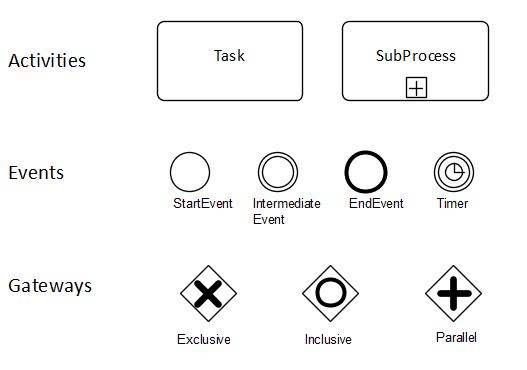
\includegraphics[width=.8\textwidth]{figuras/bpmn.png}
\caption{Principais elementos de um processo de acordo com o padrão BPMN.}
\label{fig:bpmn}
\end{figure}

Uma \emph{Activiti} é a menor parte de um diagrama BPM, e é utilizada quando o diagrama não pode ser dividido mais detalhadamente. Quando uma \emph{Activiti} está inserida no contexto de um processo, ela é chamada de \emph{Task}. Geralmente as Tasks são executadas por um usuário final ou por uma aplicação. Existem diferentes tipos de Tasks para representar os diferentes comportamentos que cada tarefa pode representar. Por exemplo, uma \emph{userTask} representa uma tarefa em que um usuário deve executar uma ação. Um elemento do tipo \emph{SubProcess} é uma abstração de um pequeno conjunto de \emph{Tasks}.
%represent. The list of Task types MAY be extended along with any corresponding indicators. \emph{userTask},\emph{manualTask}.

%events
Um \emph{Event} é algo que "acontece" durante o curso de um processo\cite{model2011notation}. Existem três tipos principais de eventos: \emph{Start Event} (indica o início do processo), \emph{End Event} (indica um fim do processo) e \emph{Intermediate Events} (indica um evento entre o início e o fim do processo).

%gateways
\emph{Gateways} são usados para controlar o fluxo do processo. Em gateways do tipo \emph{Exclusive}, apenas um dos fluxos que partem do gateway poderão ser seguidos, já em gateways do tipo \emph{Inclusive} um ou mais fluxos podem ser seguidos. Em gateways do tipo \emph{Parallel} todos os fluxos são tomados em paralelo.

%A Parallel Gateway is used to synchronize (combine) parallel flows and to create parallel flows.? The Parallel Gateway MUST use a marker that is in the shape of 
%plus sign and is placed within the Gateway
%diamond (see Figure 10.110) to distinguish it from other Gateway

%sequence flows
Um elemento \emph{Sequence Flow} é usado para exibir a ordem em que os demais elementos são executados em um processo. Cada \emph{sequenceFlow} possui apenas possui apenas uma fonte e um alvo. Analisando os elementos \emph{sequenceFlow} é possível identificar todo o fluxo do processo.

\subsection{BPM e Teste}

Os sistemas BPM geralmente oferecerem recursos para definição e modelagem de processos em BPMN, controle da execução e monitoramento de atividades dos processos~\cite{forrester}. Nota-se, no entanto, que a preocupação com testes não fica evidente nas ferramentas BPMS. De fato, examinando-se o material promocional e a documentação disponível sobre os principais BPMS, observa-se uma ênfase em etapas de modelagem e execução. Visivelmente, tais recursos são um diferencial no desenvolvimento de aplicações de BPM, em comparação ao desenvolvimento de software em geral. No entanto, aplicações de BPM também estão sujeitas a defeitos e, por isso, podem se beneficiar de avanços na área de testes de software.

Existem trabalhos que chamam a atenção para a importância e para a as dificuldades trazidas pela execução de testes, bem como trazem alternativas para a melhoria da seleção de casos de teste\cite{bohmer2015genetic}. Esses trabalhos fortalecem a ideia da importância de informações para facilitar a criação de testes para processos ou sistemas BPM, no entanto, os trabalhos geralmente abordam a criação de casos de teste baseados em modelos de processo e não em sistemas em si, não é descrita uma forma de automatizar ou executar os casos de teste criados. Existem também trabalhos que visam maneiras de automatizar e melhorar o monitoramento da conformidade dos modelos de processos \cite{ly2015compliance,van2012replaying} e que, novamente, são mais voltados para os processos em si e sua administração do que para sistema/software.

\section{Descrição da abordagem}
O objetivo deste trabalho é melhorar e facilitar o teste funcional automatizado de aplicações BPM. Um aspecto importante para o teste funcional são quais fluxos ou etapas serão testadas, pois estes podem definir ou limitar o teste, interferindo assim na qualidade e na cobertura dos testes. No entanto, a construção dessas informações pode ser uma tarefa complexa.

Com o objetivo de obter maiores informações que pudessem auxiliar no processo de teste, decidiu-se analisar os arquivos XML no formato BPMN exportados pelas ferramentas BPMS para extrair destes arquivos informações úteis. Para tratar essas informações, optou-se por analisar o processo de modo a transforma-lo em uma tabela contendo todos os possíveis fluxos que podem ser executados no processo para então serem realizadas as devidas análises. 

\begin{figure}[ht]
\centering
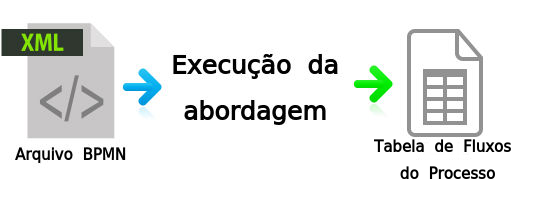
\includegraphics[width=.8\textwidth]{figuras/abordagem1.png}
\caption{Visão geral da abordagem utilizada}
\label{fig:abordagem1}
\end{figure}

Para analisar os arquivos foi elaborada um estratégia que percorre os arquivos XML e manipula as informações necessárias. A visão geral da abordagem pode ser vista na Figura \ref{fig:abordagem1}. Basicamente, o arquivo BPMN é utilizado como entrada e, enquanto o arquivo é percorrido, os elementos são analisados através da nomenclatura padrão das \emph{tags} e então é executada uma lógica para criar os diferentes cenários de teste. Ao fim da execução, é gerado um arquivo Excel contendo uma tabela com os todos os possíveis cenários/fluxos do processo.

%colcoar imagem aqui

\subsection{Funcionamento da estratégia criada}

%O principal elemento para o funcionamento da ferramenta é o \emph{Sequence Flow}. Por conter os atributos targetRef e sourceRef os elementos deste tipo permitem percorrer todo o diagrama. Ao iniciar a execução, é solicitado ao usuário o caminho para o arquivo BPMN e a ID do processo a ser avaliado. Um diagrama pode conter mais de um processo e, nesse caso, o usuário pode escolher que todos processos sejam avaliados.

Nesta abordagem, foi utilizada a linguagem Java, principalmente por esta linguagem já possuir uma opção sólida para a análise de documentos XML\cite{javadom}. O elemento BPMN mais importante para esta estratégia de análise é o \emph{Sequence Flow}. Cada \emph{Sequence Flow} possui um atributo \emph{sourceRef} que indica de onde este \emph{sequenceFlow} vem, ou sua "fonte", e um atributo \emph{targetRef} que indica para onde ele vai, ou seja, seu alvo. Por conter esses atributos os elementos deste tipo permitem percorrer todo o diagrama. Ao iniciar a execução, é solicitado ao usuário o caminho para o arquivo BPMN e a ID do processo a ser avaliado. Um diagrama pode conter mais de um processo e, nesse caso, o usuário pode escolher que todos processos sejam avaliados.

Foi criada a classe \emph{Node} que define um tipo de objeto que guarda informações básicas sobre as tarefas do processo e um \emph{array} de objetos da mesma classe. Durante a execução, um \emph{array} de objetos da classe Node é preenchido formando assim um \emph{array} de adjacências. O método principal percorre o processo recursivamente através dos elementos do tipo \emph{Sequence Flow}, enquanto um tarefa for encontrada, um objeto da classe Node é criado e o método é chamado recursivamente de modo a retornar o \emph{array} de adjacências para este objeto.

A partir do \emph{array} de adjacências são criados os fluxos possíveis pelos quais o processo pode passar. O método que cria os fluxos percorre recursivamente o \emph{array} de adjacências criado anteriormente e "constrói" um novo fluxo possível, tendo como condição de parada o encontro de uma das últimas tarefas a serem executadas. Uma tarefa é uma das últimas quando o elemento que a sucede no fluxo for elemento do tipo\emph{End Event}. Ao encontrar uma tarefa final, a informação é armazenada e é iniciada a construção de um novo fluxo possível.

Os fluxos obtidos são base para a criação da tabela. Para criar a tabela, cada tarefa existente no processo representará uma coluna na tabela e cada fluxo representará uma nova linha. Para cada fluxo, se a tarefa estiver presente a coluna será marcada com "X" caso contrário a coluna será marcada com um "0". Caso mais de um processo seja avaliado ao mesmo tempo, a tabela referente à cada processo estará separada individualmente no arquivo final. 

Na Tabela \ref{tab:exemplo}, pode ser visto uma tabela resultante da execução dessa estratégia para um processo com cinco \emph{tasks} e dois fluxos possíveis. Com a geração desta tabela podem ser realizadas diversas análises sobre o processo: número de fluxos possíveis, identificar gargalos, etc.

\begin{table}[]
\centering
\caption{Exemplo de tabela resultante}
\label{tab:exemplo}
\begin{tabular}{ccccc}
\multicolumn{1}{l}{Quotation Handling} & \multicolumn{1}{l}{Approve Order} & \multicolumn{1}{l}{Order Handling} & \multicolumn{1}{l}{Shipping Handling} & \multicolumn{1}{l}{Review Order} \\
X & X & 0 & 0 & 0 \\
X & X & X & X & X
\end{tabular}
\end{table}

\subsection{Dificuldades/Limitações}
A maioria das dificuldades encontradas são relacionadas à estrutura dos processos e como a implementação interpretaria essas características. Na criação dos fluxos possíveis, uma dificuldade ocorreu devido aos desvios causados por elementos do tipo \emph{Gateway}. Para isso, para cada Node criado no \emph{array} é guardado o tipo do elemento que o antecede. Assim, na criação dos fluxos, elementos que partem de um desvio de fluxo precisaram ser tratados para criar os fluxos corretamente, por exemplo: se dois elementos, X e Y, vem de um \emph{gateway} do tipo  exclusivo, os fluxos obtidos até estes elementos serão duplicados, ou seja, metade dos fluxos passaram apenas por X e metade dos fluxos passarão apenas por Y.

%Na criação dos fluxos, há uma exceção para quando existir uma divisão de fluxo através de um gateway do tipo inclusivo. Diferente do que acontece com o tipo exclusivo, onde apenas uma opção de pode ser seguida de cada vez, no \emph{gateway} inclusivo as opções podem variar pois um ou mais fluxos podem ser seguidos ao mesmo tempo. Os casos em que apenas um fluxo é seguido já são cobertos pela execução normal do parser, então, após a criação dos fluxos, é identificada a existencia de casos inclusivos e, se necessário, fluxos adicionais são inseridos.

Devido ao fato da estratégia implementada ser executada recursivamente e percorrer o processo baseado no fluxo dos elementos do tipo \emph{SequenceFlow}, ocorreram problemas em processos onde uma parcela do processo também é executada recursivamente. Estes problemas foram causados devido ao fluxo nunca encontrar um "fim". Para solucionar esses problema foi criado um "delimitador de recursão" que define e controla o número de vezes em que o mesmo \emph{SequenceFlow} será executado.

Algumas ferramentas exportam o diagrama para o formato BPMN inserindo um ``tipo'' antes no nome de cada tag XML, por exemplo, a \emph{tag} de nome \emph{task} pode estar representada como ``semantic:task'' e isso pode impedir que o parser XML do Java identifique os elementos. Assim, foi necessário preparar métodos para tratar este tipo de situação removendo os elementos encontrados antes dos nomes de \emph{tags}.

%Na criação dos artefatos para o teste funcional são levados em conta apenas tarefas que podem ser executadas por um usuário. 
Apesar de utilizarem o mesmo padrão BPMN, algumas ferramentas podem utilizar nomes diferentes para representar tarefas no arquivo XML. Por isso, dependendo do BPMS que for utilizado, pode ser necessário substituir o nome das tarefas tratadas diretamente no código.

%pode gerar fluxos iguais, por remover boa parte das tarefas, como pdoe ser visto na figura de antes também

%-subprocess -> apenas como uma tarefa, normalmente sao simples, so testa o principal,subprocessos normalmente sao simples


\section{Teste Funcional de Software e um exemplo de uso da abordagem}
O teste funcional é um tipo de teste que permite verificar as saídas de um sistema produzidas a partir de entradas pré-definidas. Este tipo de teste permite testar as funcionalidades, requerimentos e regras de negócio presentes no software\cite{molinari2003testes} verificando a existência de erros, o que auxilia na melhoria da qualidade do software.

Uma das principais medidas para o teste de software é a cobertura de teste. A cobertura de teste mede a abrangência do teste e pode ser expressa pela cobertura dos casos de testes ou pela cobertura do código executado. Existem diversos trabalhos que abordam a importância da cobertura de testes de software\cite{zhu1997software,bieman1996using}, inclusive ligando o crescimento da qualidade e confiabilidade do software ao crescimento da cobertura dos testes\cite{malaiya2002software}.


No entanto, as atividades executadas para criar testes funcionais com uma boa cobertura podem muitas vezes se tornar exaustivas e trabalhosas, dificultando assim a execução dos testes de forma adequada. Com o objetivo de melhorar a qualidade da análise e o tempo de execução dos testes, foram criados os testes automatizados, que proporcionam a execução dos testes mais rapidamente \cite{fantinato2005autotest}. Quando executada corretamente, a automação de teste é uma das melhores formas de reduzir o tempo de teste no ciclo de vida do software, diminuindo o custo e aumentando a produtividade do desenvolvimento de software como um todo, além de, consequentemente, aumentar a qualidade do produto final.

Para executar os testes funcionais automatizados em aplicações Web, pode-se utilizar ferramentas livres como Selenium\cite{selenium}, Watir\cite{watir} ou Geb\cite{geb}. No trabalho anterior\cite{sbqs2015}, onde os testes funcionais se mostraram mais promissores, foi utilizada a ferramenta Selenium, aliada ao Cucumber-JVM\cite{cucumber} para descrição dos testes. A escolha foi motivada pelo grande número de referências ao Selenium na Web, confirmadas por um trabalho que apresentou resultados satisfatórios com Selenium e Cucumber\cite{pannutest,sbqs2013}.

\subsection{Teste Funcional Automatizado utilizando \emph{Selenium} e \emph{Cucumber-JVM}}
O processo para a execução de um teste funcional utilizando o Selenium aliado ao Cucumber-JVM é composto de cinco etapas: captura da interação do usuário com a aplicação e exportação do código gerado, criação dos cenários de teste, criação das definições dos passos de teste, implementação dos métodos para cada passo e, por fim, execução do teste.

Para efetuar a captura da interação do usuário com a aplicação é utilizado o Selenium IDE (\emph{Integrated Development Environment}), que permite gravar as ações do usuário conforme elas são executadas. Assim, a funcionalidade que deseja ser testada deve ser executada para que os passos sejam gravados. Após a captura da interação é possível exportar o \emph{script} utilizando diversas linguagens de programação disponíveis, neste caso foi escolhida a linguagem Java.

Os testes utilizando o Cucumber são compostos, basicamente, por dois arquivos: arquivos que especificam as funcionalidades \emph{features} e por arquivos de definição de passos \emph{steps}. 

Os arquivos com as funcionalidades são escritos utilizando a linguagem Gherkin\cite{gherkin} e são compostos por cenários, os cenários representam uma fração da aplicação que vai ser testada. Um cenário também pode ser descrito como a definição, em ordem de execução, das etapas que são executados nessa fração, bem como dos resultados esperados para validar a aplicação. Por exemplo, após um \emph{gateway} exclusivo com dois fluxos disponíveis, já é possível obter dois cenários possíveis: um cenário executando cada fluxo.
%Por exemplo, para testar apenas o login em uma aplicação, já é possível obter dois cenários possíveis: (a) dados de acessos corretos e sucesso no login e (b) dados de acesso incorretos e mensagem de erro. 

Para que cada etapa do cenário seja executada, é necessária a criação de \emph{steps} que irão traduzir os passos definidos na linguagem Gherkin para ações que vão interagir com o sistema. Cada \emph{step}, geralmente, irá chamar um método Java que irá efetivamente executar a interação com a aplicação. A implementação destes métodos pode ser feita apenas utilizando o código extraído através do Selenium após a captura das ações do usuário.

Assim, mesmo utilizando o Cucumber e Selenium para facilitar a criação dos testes, ainda é preciso analisar o processo e extrair os cenários de teste que devem ser criados manualmente no arquivo de \emph{features}. Além dos cenários, também deve ser criado manualmente o arquivo de \emph{steps}, contendo uma "passo" correspondente a cada etapa de todos os cenários criados. Esta etapa pode ser trabalhosa, principalmente quando for necessário testar todos diversos cenários que um processo pode ter ou quando o processo for extenso.

\subsection{Uma opção de uso da ferramenta: criação dos elementos utilizados no teste funcional}
A geração da tabela com informações relevantes para o teste do processo foi a principal motivação da criação da ferramenta. No entanto, além das análises que a própria tabela possibilita, também é possível utilizar a ferramenta criada para gerar outros elementos conforme a necessidade de cada domínio. No caso deste trabalho, por o teste funcional automatizado utilizando o Selenium e o Cucumber se mostrou promissor em um trabalho anterior \cite{sbqs2015}, decidiu-se por avaliar a possibilidade de aproveitar a ferramenta criada para também gerar elementos importantes para o teste: o arquivo de \emph{features} contendo os cenários cenários e o arquivo de \emph{steps}.

\begin{figure}[ht]
\centering
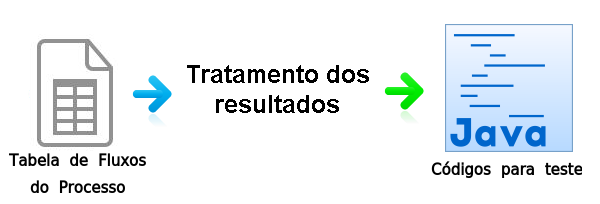
\includegraphics[width=.9\textwidth]{figuras/abordagem2.png}
\caption{Uma das opções de uso da abordagem: geração de códigos para o teste funcional}
\label{fig:abordagem2}
\end{figure}

O arquivo contendo os cenários de teste é essencial para o teste funcional com o Cucumber, no entanto a criação dos arquivos de \emph{features} contendo os cenários e do arquivo de \emph{steps} pode ser trabalhosa, como foi mencionado na seção anterior. Uma visão geral deste exemplo de uso pode ser vista na Figura \ref{fig:abordagem2}, onde a tabela resultante da execução da abordagem é utilizada para gerar os arquivos com códigos. Para criar estes elementos, foram adicionadas algumas funcionalidades na ferramenta para que os dados já obtidos fossem tratados. Assim, cada fluxo que foi obtido pela ferramenta, e consta na tabela de saída, foi considerado um cenário diferente. Como trata-se de um teste funcional, apenas tarefas que podem ser executadas por um usuário foram ser avaliadas (\emph{userTask},\emph{manualTask}...). Assim, para cada fluxo é criado um novo cenário no arquivo de \emph{features} utilizando a notação do Cucumber e contemplando apenas as tarefas que podem ser executadas por um usuário. O método correspondente a cada passo do cenário é criado ao mesmo tempo e inserido no arquivo de \emph{steps}. %Na Figura \ref{fig:exemplo_cenario}, podem ser vistos dois cenários resultante da execução do parser para um processo com dois fluxos possíveis. 

%colocar código aqui
%\begin{figure}[ht]
%\centering
%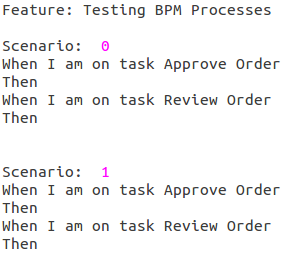
\includegraphics[width=.5\textwidth]{figuras/exemplo_cenario.png}
%\caption{Exemplo de cenários resultantes}
%\label{fig:exemplo_cenario}
%\end{figure}

\section{Avaliação}
Para avaliar a ferramenta foram buscados processos já existentes, de diferentes domínios, contendo ao menos três tarefas e uma divisão de fluxo com ou sem \emph{gateway}, também era interessante que os processos selecionados tivessem algumas diferenças de notação para verificar como a ferramenta trataria essas diferenças. Assim, os processos utilizados para a validação foram obtidos no site da \emph{Object Management Group} (OMG) e estão disponíveis no \href{http://www.omg.org/spec/BPMN/20100602/2010-06-03/}{site} da organização.

 %A Tabela \ref{tab:resumoprocessos} apresenta uma visão geral dos processos avaliados, as informações referentes ao número de tarefas e de fluxos foram extraídas das tabelas obtidas após executar a abordagem para cada processo. Na Tabela \ref{tab:resumoprocessos}, podemos ver que a divisão de fluxos é importante para os testes pois ela delimita quantos fluxos existem no processo, ou seja, quantos fluxos podem ser testados. 
 
 %Outro ponto importante é que, em alguns casos, podem existir divisão de fluxo sem \emph{gateways}. As divisões sem \emph{gateways}, dependendo da ferrmaneta BPMS utilizada para gerar o processos podem ser visualizadas só analisando o documento xml o que atrapalha a analise no9 entanto a abordagem permite que essas divisões sejam detectadas e tratadas automaticamente

\begin{table}[]
\centering
\caption{Resumo dos processos avaliados}
\label{tab:resumoprocessos}
\begin{tabular}{cccc}
Número de tarefas & Número de Gateways & Tipo do Gateway                 & Fluxos possíveis \\
3                 & 0                  & Sem divisão de fluxos           & 1                \\
3                 & 1                  & Exclusivo                       & 2                \\
4                 & 0                  & Divisão de fluxos sem Gateways  & 2                \\
5                 & 0                  & Divisão de fluxos sem Gateways  & 3                \\
5                 & 1                  & Exclusivo                       & 3                \\
6                 & 2                  & Exclusivo                       & 3                \\
7                 & 1                  & Exclusivo                       & 2                \\
8                 & 3                  & Inclusivo, Exclusivo e Paralelo & 3                \\
8                 & 3                  & Paralelo, Exclusivo e Inclusivo & 6                \\
10                & 1                  & Exclusivo                       & 2
\end{tabular}
\end{table}

\begin{figure}[ht]
%\centering
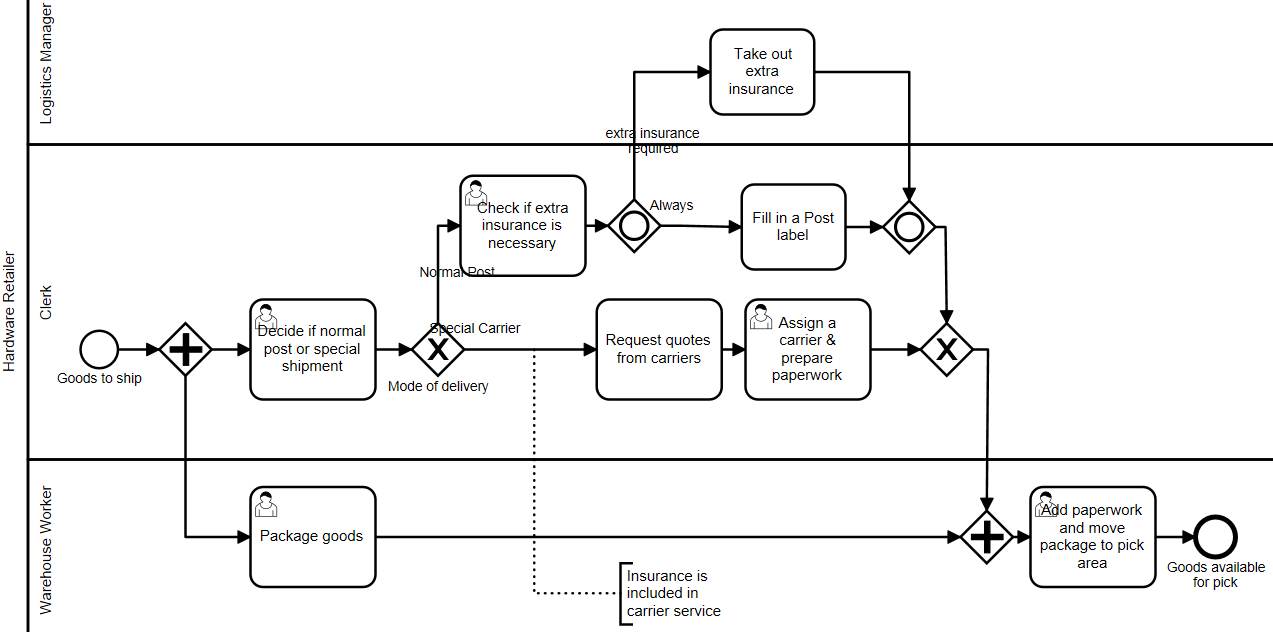
\includegraphics[width=.9\textwidth]{figuras/diagrama_exemplo.png}
\caption{Exemplo de Processo. Adaptado de: Object Management Group}
\label{fig:diagrama_exemplo}
\end{figure}

%gera a tabela com os caminhos
%identificar: gargalos, quais tarefas são mais executadas, quais caminhos são mais criticos
%como gera o código para todos, pode testar todos ou selecionar através da tabela gerada os caminhos mais importante e utilizar o código referente só a aqueles caminhos

Com a análise do arquivo BPMN através da ferramenta criada foi possível obter um elemento importante para o teste funcional de aplicações BPM: a tabela relacionando as tarefas e os fluxos possíveis dentro de um processo. Por exemplo, o processo na Figura \ref{fig:diagrama_exemplo} possui \emph{gateways} de diferentes tipos, gerando assim várias divisões de fluxo e aumentando os fluxos que podem ser seguidos. 

%analise da tabelinha (que consegue gargalo...blabla)
Ao executar a ferramenta utilizando o arquivo BPMN referente ao processo da Figura  \ref{fig:diagrama_exemplo} foi obtida a Tabela \ref{tab:resultado}. Nesta tabela, cada coluna representa uma tarefa do diagrama e cada linha representa um fluxo possível, facilitando a visualização do processo. 

\begin{table}[]
\centering
\caption{Tabela obtida através do arquivo BPMN}
\label{tab:resultado}
\resizebox{\textwidth}{!}{%
\begin{tabular}{cccccccc}
%Decide if normal post or special shipment & Request quotes from carriers & Assign a carrier \& prepare paperwork & Check if extra insurance is necessary & Take out extra insurance & Fill in a Post label & Package goods & Add paperwork and move package to pick area \\
Decide if normal... & Request quotes... & Assign a carrier \& prepare paperwork & Check if extra... & Take out extra insurance & Fill in a Post label & Package goods & Add paperwork and...\\
X & X & X & 0 & 0 & 0 & X & X \\
X & 0 & 0 & X & X & 0 & X & X \\
X & 0 & 0 & X & 0 & X & X & X \\
X & 0 & 0 & 0 & 0 & 0 & X & X \\
X & 0 & 0 & X & X & X & X & X
\end{tabular}%
}
\end{table}

A criação da tabela diminui o tempo de análise dos processos e também torna o teste mais completo ao mesmo tempo em que verifica todos os possíveis fluxos que um processo pode seguir. A tabela criada também permite análises de diversos fatores importantes para a execução dos processos como: gargalos, quais tarefas poderão ser mais frequentemente executadas, entre outros. Por exemplo, na Tabela \ref{tab:resultado} pode-se dizer que a primeira e as duas últimas tarefas do processo são gargalos, pois todas os fluxos possíveis passarão por essas tarefas. 

Como uma das opções possíveis de aproveitamento da informação obtida na tabela extraída, nesse trabalho abordamos a criação de códigos para teste funcional do processo utilizando as ferramentas de automação Selenium e Cucumber-JVM. Para executar o teste completo do processo, testando todas as possibilidades e representando as informações obtidas na tabela, seria necessário planejar os cenários de teste e criá-los manualmente. Para criar os cenários também é necessário identificar quais tarefas são executadas por um usuário em um processo que possui várias \emph{tasks}. Por fim, também seria necessário criar os \emph{steps} para cada etapa do cenário manualmente.
 


Executando o parser criado utilizando o arquivo BPMN referente ao diagrama da Figura \ref{fig:diagrama_exemplo} como exemplo, obtemos os cenários de teste representados no trecho de código abaixo. 


\begin{lstlisting}[language=Java]
Feature: Testing BPM Processes  
 
Scenario: Hardware Retailer 0 
Given I am on task Decide if normal post or special shipment 
When 
Then 
When I am on task Assign a carrier & prepare paperwork 
Then 
When I am on task Add paperwork and move package to pick area 
Then 
 
Scenario: Hardware Retailer 1 
Given I am on task Decide if normal post or special shipment 
When 
Then 
When I am on task Check if extra insurance is necessary 
Then 
When I am on task Add paperwork and move package to pick area 
Then 
 
Scenario: Hardware Retailer 2
When I am on task Package goods 
Then 
When I am on task Add paperwork and move package to pick area 
Then 

\end{lstlisting}

Para o teste funcional do processo em questão, três cenários são possíveis, representando as duas principais divisões de fluxo encontradas no processo. A primeira divisão de fluxo formada pelo \emph{gateway} do tipo paralelo logo no início do processo, está contida no cenário de forma que os cenários \emph{Hardware Retailer 0} e \emph{Hardware Retailer 1} fazem parte de um fluxo e o cenário \emph{Hardware Retailer 2} representa o segundo fluxo possível. A segunda divisão de fluxo no processo da Figura \ref{fig:diagrama_exemplo} é formada pelo \emph{gateway} do tipo exclusivo, e essa divisão é representada pelos cenários \emph{Hardware Retailer 0} e \emph{Hardware Retailer 1}. Há ainda uma terceira divisão de fluxo no processo, esta divisão não foi levada em conta pelo parser pois as tarefas subsequentes a essa divisão não são tarefas executadas pelo usuário.

%Como foi mencionado anteriormente, apenas tarefas executadas por usuários são levadas em conta para o teste funcional, e por isso nem todas as tarefas do processo estarão presentes nos cenários de teste.


Para cada etapa nos cenários criados será criado um método correspondente dentro do arquivo de \emph{steps} chamado \emph{stepDefinition}. Uma parte do arquivo de \emph{steps} resultante da análise do processo em questão pode ser visto no trecho de código abaixo. Como pode ser visto neste codigo, para a etapa de cenário chamada \emph{I am on the task Decide if normal post or special shipment} foi criado um método com um nome genérico e contendo a anotação \emph{@Given("\^{}I am on the task Decide if normal post or special shipment\textdollar{}")}. Os métodos podem ser preenchidos posteriormente com os dados gravados pelo Selenium na etapa de captura da interação com a aplicação.

\begin{lstlisting}[language=Java]
import cucumber.api.java.en.*;
import cucumber.runtime.PendingException;
public class StepsDefinition{
@Before
public void beforeScenario(){}
@After
public void afterScenario(){} 
//Methods for process Hardware Retailer
@Given("^I am on the task Decide if normal post or special shipment$") 
public void method0() throws Exception {} 
@when("^name$") 
public void method1() throws Exception {} 
@Then("^name$") 
public void method2() throws Exception {} 
@When("^I am on the task Assign a carrier & prepare paperwork$") 
public void method3() throws Exception {} 
\end{lstlisting}


%\begin{itemize}
%\item Exemplo de processo, Figura \ref{fig:diagrama_exemplo};
%item Exemplo dos artefatos obtidos: tabelinha e cenário de teste (apenas necessário completar com os códigos obtidos no selenium)
%	\item Melhoria na criação dos testes (mais rápido e mais completo);
%	\item Por consequência: Melhoria na cobertura dos testes (todos fluxos e cenários possíveis)
%	\item Por consequência: auxilia na melhora da qualidade dos sistemas.
%\end{itemize}

Neste exemplo, apenas um processo foi analisado, mas arquivos BPMN podem conter vários processos. Neste caso, se for necessário gerar os dados para todos os processos dentro de um arquivo, o arquivo contendo a tabela resultante será composto por várias tabelas, uma para cada processos analisado, agilizando ainda mais a obtenção das informações. 




Foi possível obter uma tabela importante para analise dos processo, permitindo que sejam obtidas muitas informações úteis e importantes para a execução de testes completos e com boa cobertura. Como um exemplo de utilização das informações obtidas foram gerados dois arquivos essenciais para o teste funcional automatizado de aplicações BPM: o arquivo com os cenários de teste e o arquivo com os métodos para executar cada etapa dos cenários.

\section{Conclusão}

O objetivo desse trabalho foi melhorar e facilitar o teste funcional de aplicações BPM. Foi possível obter uma tabela com todos fluxos possíveis dentro do processo. A criação da tabela possibilita a criação de testes mais completos e com boa cobertura o que, por consequência, contribui para a melhoria da qualidade das aplicações. A tabela gerada também permite que sejam feitas análises importantes sobre o processo como, por exemplo, identificar gargalos.

Além da obtenção da própria tabela, a abordagem permite que as informações sejam usadas como entrada na criação de outros elementos. As informações podem ser reutilizadas das mais diversas formas, nesse trabalho decidiu-se por abordar como uma das opções o teste funcional com as ferramentas Selenium e Cucumber. Em um trabalho anterior a execução do teste funcional automatizado em aplicações BPM com as ferramentas mencionados se mostrou promissora, mas trabalhosa. A abordagem utilizada auxilia nesse ponto pois permitiu que se utilizassem as informações obtidas para gerar códigos necessários para a execução dos testes, facilitando ainda mais a automação destes.

A criação automatizada da tabela e dos dois arquivos permite facilitar e melhorar a criação dos testes para os sistemas BPM, diminuindo o tempo de análise dos processos bem como tornando o teste mais completo ao mesmo tempo em que verifica todos os possíveis fluxos que um processo pode seguir. Assim, a qualidade e a cobertura dos testes também é melhorada pois todos os fluxos e cenários possíveis são analisados. Por consequência, a qualidade dos sistemas também pode ser beneficiada com um processo de teste mais completo e facilitado.

Como trabalhos futuros têm se a melhoria de alguns aspectos técnicos da abordagem como melhorar o tratamento a processos com recursão e reconhecimento dos diferentes nomes de \emph{tag}. Também podem ser avaliadas outras formas de utilizar as informações extraídas de forma a gerar outros elementos.
%\begin{itemize}
%\item Trabalhos futuros (tirar repeticoes de cenários, tentar gerar mais coisas/informações, verificar outras opções pra utilizar), criar um "dicionário" com o maior numero possível de nomes distintos para cada tag e automatizar esse interpretação
%\end{itemize}
 

\section{Referências}

\bibliographystyle{sbc}
\bibliography{sbc-template}

\end{document}

%gerando 